\documentclass[xcolor={svgnames},12pt,aspectratio=169]{beamer}
\usetheme{Berlin}
\usecolortheme{dolphin}

\setbeamercolor*{structure}{bg=Azure,fg=MidnightBlue!50!black}

\setbeamercolor*{palette primary}{use=structure,fg=structure.bg,bg=structure.fg}
\setbeamercolor*{palette secondary}{use=structure,fg=structure.fg,bg=structure.bg}
\setbeamercolor*{palette tertiary}{use=structure,fg=structure.fg,bg=GhostWhite}
\setbeamercolor*{palette quaternary}{fg=white,bg=black}

\setbeamercolor{section in head/foot}{parent=palette primary} % Outer section of header/footer
\setbeamercolor{subsection in head/foot}{parent=palette secondary} % Inner section of header/footer

\setbeamercolor{titlelike}{parent=palette tertiary} % Main titles
\setbeamercolor{frametitle}{parent=palette tertiary,bg=GhostWhite!50}

\setbeamercolor{section in toc}{fg=darkgray,bg=Azure} % Table of contents sections
\setbeamercolor{subsection in toc}{fg=darkgray,bg=Azure} % Table of contents subsections
% \setbeamercolor{alerted text}{use=structure,fg=structure.fg!50!black!80!black}

% \setbeamertemplate{navigation symbols}{} % Hides navigation buttons at the bottom
% \setbeamertemplate{headline}{} % Hides navigation bar at the top

\setbeamercovered{transparent}

\setbeamertemplate{caption}[numbered]

% \usepackage{pgfpages}
% \pgfpagesuselayout{4 on 1}[a4paper,border shrink=5mm]

\usepackage[utf8]{inputenc}
\usepackage{adjustbox}
\usepackage{xcolor,colortbl}
\usepackage[all]{xy}
\usepackage{tikz}
\usetikzlibrary{mindmap,backgrounds}
\usepackage{graphicx}
\usepackage{multicol}
% Advanced table functions
\usepackage{tabularx,ragged2e}
\usepackage{booktabs}
% Listings extension
\usepackage{listings}

\title[Empowering Users' Privacy Rights in the Internet of Things]{Master's Thesis Preparation \\ {\normalsize Empowering Users' Privacy Rights in the Internet of Things}}
% \subtitle{Empowering Users' Privacy Rights in the Internet of Things}
\author{\href{mailto:2080511@student.uma.pt}{Nelson Vieira}
% \\ \and \href{mailto:mary.barreto@staff.uma.pt}{Mary Barreto (advisor)}
}
\institute[\href{https://www.uma.pt/}{University of Madeira}]{University of Madeira\\Faculty of Exact Sciences and Engineering}
\date{Last Update: \today}

\setbeameroption{show notes}

\makeatletter
    \newenvironment{withoutheadline}{
        \setbeamertemplate{headline}[default]
        \def\beamer@entrycode{\vspace*{-\headheight}}
    }{}
\makeatother

\begin{document}

\begin{withoutheadline}
    \begin{frame}
        \centering
\includegraphics[width=100pt]{../assets/images/uma_logo.png}
        \maketitle
    \end{frame}
\end{withoutheadline}

\begin{frame}{Table of Contents}
    % Use hideallsubsections for longer presentations
    % \tableofcontents[hideallsubsections]
    \begin{multicols}{2}
        \tableofcontents
    \end{multicols}
\end{frame}

\section{Introduction}

\begin{frame}{Introduction}
    Internet of things (IoT) devices are everywhere. These devices
    create new ways of collecting and process personal data from users and
    non-users. Most end users are not even aware or have little control over
    the information that is being collected by these systems.

    This work takes an holistic approach to this problem by doing:
    \begin{itemize}
        \item<2-> Systematic literature review;
        \item<3-> A survey;
        \item<4-> A mobile application.
    \end{itemize}
\end{frame}

\begin{frame}{Privacy}
    \begin{multicols}{2}
        What is privacy?
        \begin{figure}
            \centering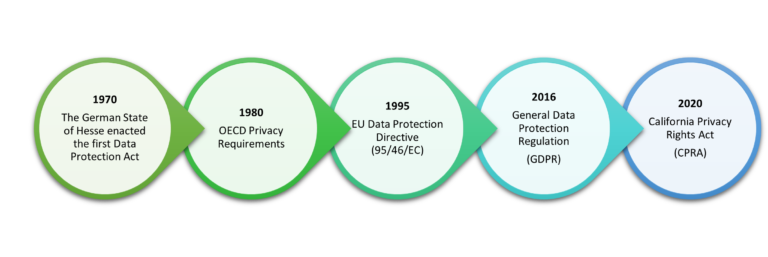
\includegraphics[width=200pt]{assets/images/privacy_history.png}
            \caption{Privacy history \cite{MukherjeePrivacy}}
        \end{figure}

        \columnbreak
        % \onslide*<2>
        \centering
        \vspace*{\fill}
        Privacy $\ne$ Security
        \vspace*{\fill}
    \end{multicols}
\end{frame}

\begin{frame}{Internet of Things}
    \begin{multicols}{2}
        \begin{figure}
            \centering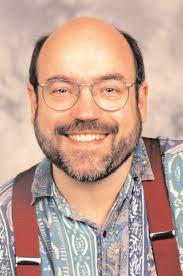
\includegraphics[width=80pt]{assets/images/mark_weiser.png}
            \caption{Mark Weiser \cite{weiser1991computer}}
        \end{figure}

        \columnbreak
        \begin{figure}
            \centering
\includegraphics[width=120pt]{assets/images/kevin_ashton.png}
            \caption{Kevin Ashton \cite{KevinThat}}
        \end{figure}
    \end{multicols}
\end{frame}

\section{State of the Art}

\subsection{Privacy Paradox}

\begin{frame}{Privacy Paradox}
    \begin{multicols}{2}
        What is it?

        \vspace*{\fill}
        Why even worry about privacy?
        \vspace*{\fill}

        \columnbreak
        \begin{figure}
            \centering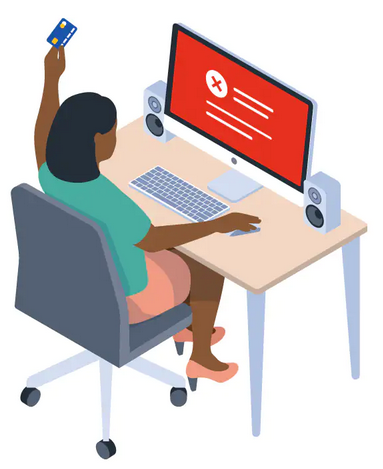
\includegraphics[width=90pt]{assets/images/privacy_paradox.png}
            \caption{How much privacy are we willing to give up online? \cite{ClareParadox}}
        \end{figure}
    \end{multicols}
\end{frame}

\subsection{Differential Privacy}

\begin{frame}{Differential Privacy}
    \begin{figure}
        \centering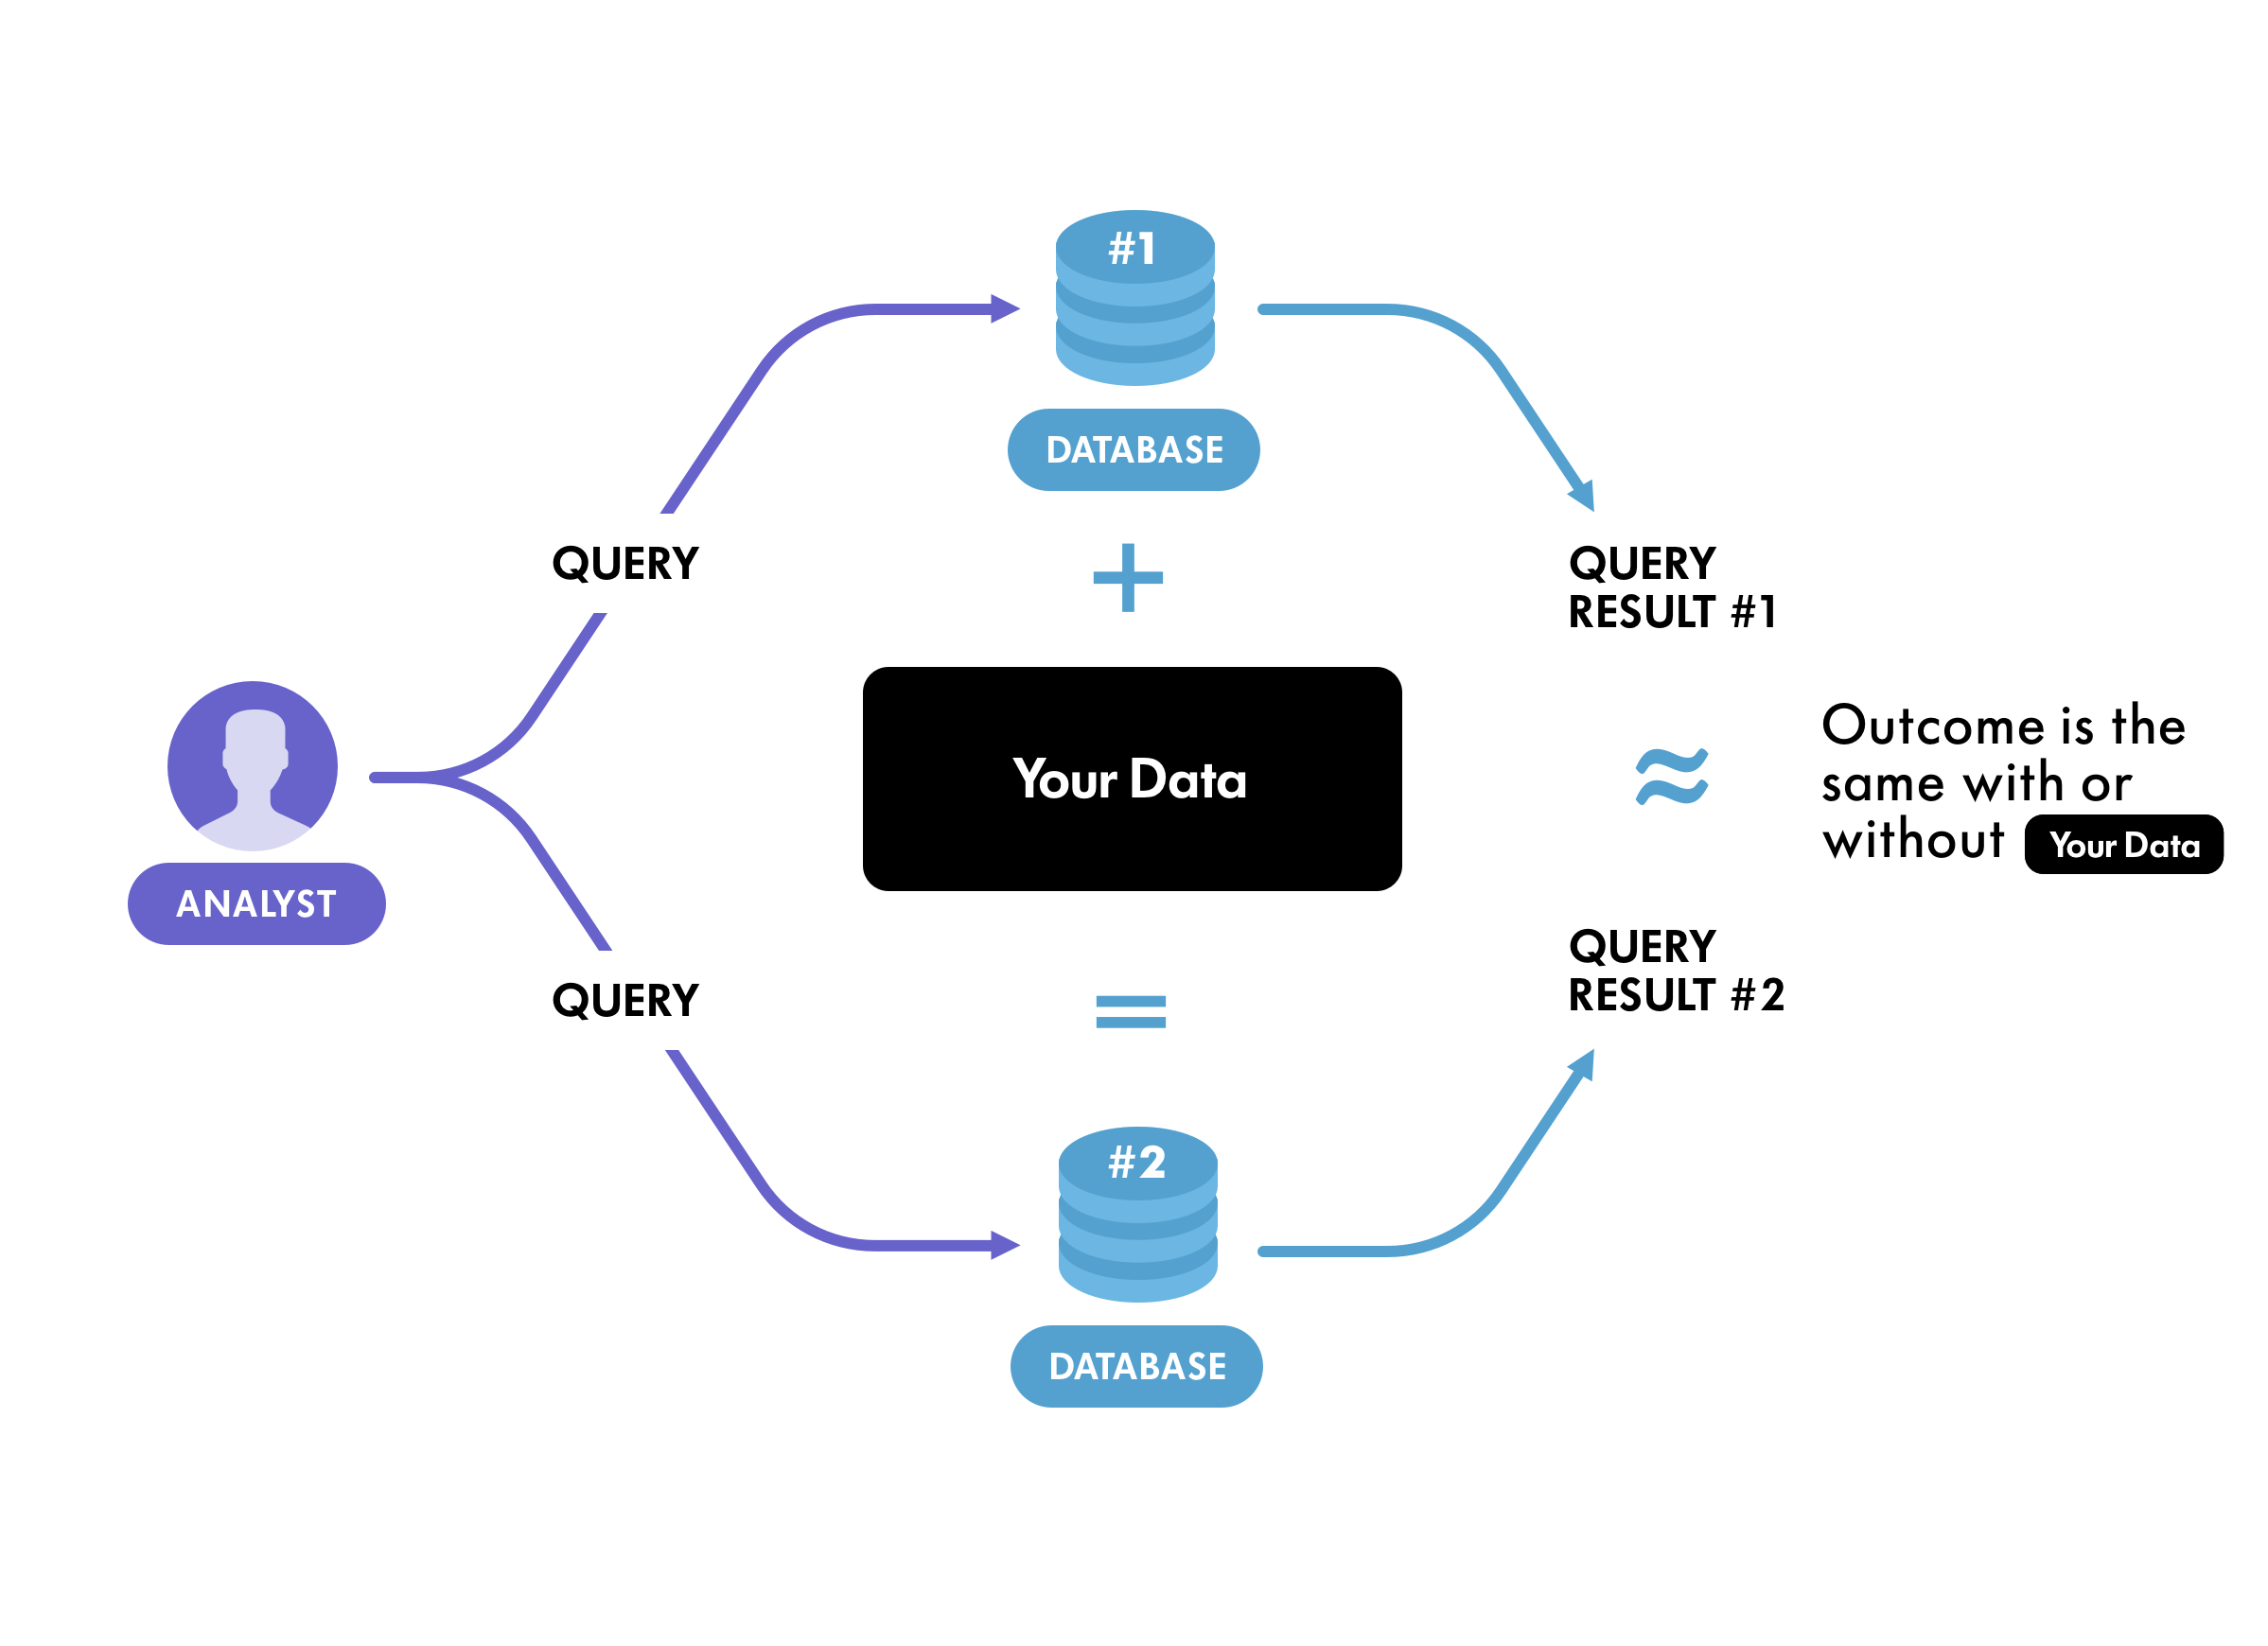
\includegraphics[width=180pt]{assets/images/dp.png}
        \caption{Differential Privacy \cite{WintonDifferential}}
    \end{figure}
\end{frame}

\subsection{Literature Approaches}

\begin{frame}{Literature Approaches}
    \begin{itemize}
        \item<1-> User awareness;
        \item<2-> Privacy through security;
        \item<3-> Framework proposals;
        \item<4-> Blockchain;
    \end{itemize}
\end{frame}

\begin{frame}{Privacy Assistants}
    \begin{multicols}{2}
        \begin{figure}
            \centering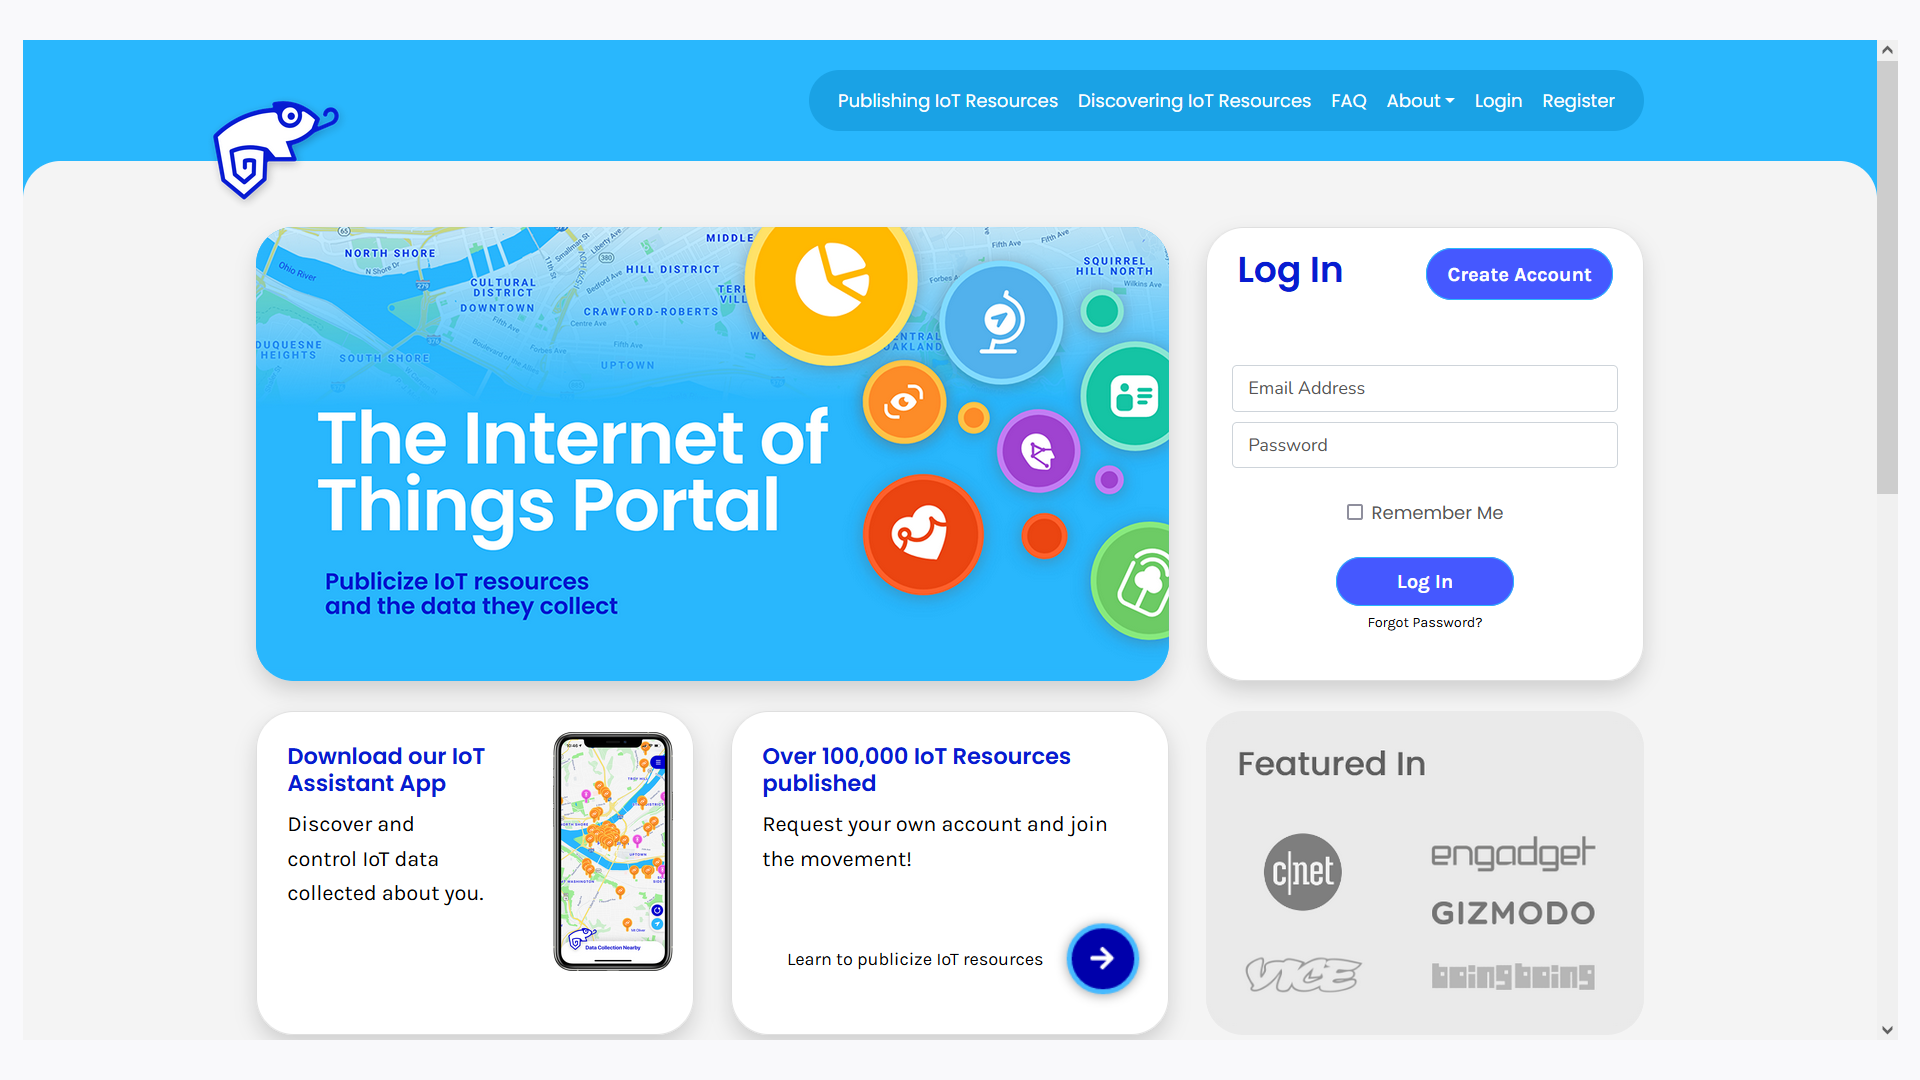
\includegraphics[width=180pt]{assets/images/iot_portal.png}
            \caption{Internet of Things Portal}
        \end{figure}

        \columnbreak
        \begin{figure}
            \centering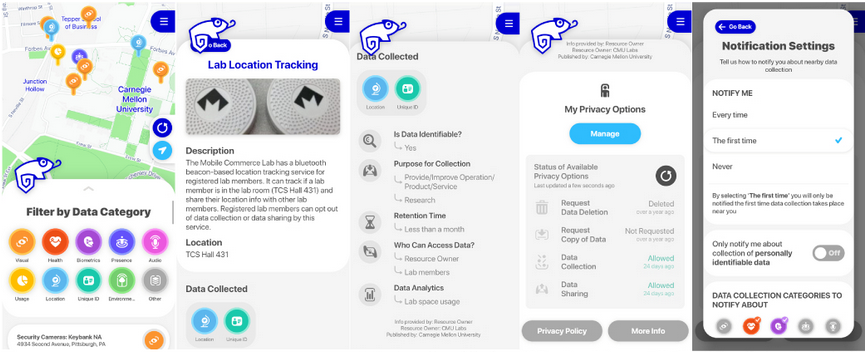
\includegraphics[width=210pt]{assets/images/iot_assistant.png}
            \caption{Internet of Things Assistant}
        \end{figure}
    \end{multicols}
\end{frame}

\section{Methodology}

\subsection{Survey}

\begin{frame}[shrink]{Survey}
    \begin{multicols}{2}
        92 Questions
        \begin{itemize}
            \item General knowledge and attitudes towards privacy
            \item Disposition for sharing personal information
            \item Privacy concerns
            \item Current online habits and practices
            \item Profile identification
            \item Knowledge and habits regarding the Internet of Things
            \item Demographic data
        \end{itemize}

        \columnbreak
        \begin{figure}
            \centering
\includegraphics[width=45pt]{assets/images/forms.png}
            % \caption{LFE channel frequency spectrum}
        \end{figure}
        \begin{figure}
            \centering
\includegraphics[width=70pt]{assets/images/mturk.jpg}
            % \caption{LFE channel frequency spectrum}
        \end{figure}
    \end{multicols}
\end{frame}

\subsection{Application}

\begin{frame}{Application}
    \begin{multicols}{2}
        Will be composed of the following things:
        \begin{itemize}
            \item Show the geolocation of the IoT devices;
            \item What type of device it is;
            \item What type of data is being collect by the device;
            \item Insert IoT devices and associated information about them.
        \end{itemize}

        \columnbreak
        \begin{figure}
            \centering
\includegraphics[width=120pt]{assets/images/flutter.png}
            % \caption{LFE channel frequency spectrum}
        \end{figure}
    \end{multicols}
\end{frame}

\section{Conclusion and Future Work}

\subsection{Future Work}

\begin{frame}{Future Work}
    \begin{table}[ht]
        \centering
        \begin{adjustbox}{width=0.9\textwidth}
        \small
        \noindent\begin{tabular}{p{0.17\textwidth}*{20}{p{0.01\textwidth}}|}
        \hline
        \multicolumn{0}{|c|}{}
            & \multicolumn{4}{c|}{January}
            & \multicolumn{4}{c|}{February}
            & \multicolumn{4}{c|}{March}
            & \multicolumn{4}{c|}{April}
            & \multicolumn{4}{c|}{May}
            \\
        % \hline
        % \hline
        \multicolumn{0}{|l|}{}
            & 1 & 2 & 3 & \multicolumn{0}{c|}{4} & 1 & 2 & 3 & \multicolumn{0}{c|}{4}& 1 & 2 & 3 & \multicolumn{0}{c|}{4}& 1 & 2 & 3 & \multicolumn{0}{c|}{4}& 1 & 2 & 3 & 4 \\
        \hline
        % using the on macro to fill in twenty cells as `on'
        \multicolumn{0}{|l|}{Discovery and planning}
            & \cellcolor[cmyk]{1,1,0,0}&&&& &&&& &&&& &&&&&&& \\
        % \hline
        \multicolumn{0}{|l|}{Research enquiry}
            & \multicolumn{12}{c}{\cellcolor[cmyk]{1,1,0,0}} &&&& &&&& \\
        % \hline
        \multicolumn{0}{|l|}{State of the art}
            & \multicolumn{8}{c}{\cellcolor[cmyk]{1,1,0,0}} &&&& &&&& &&&& \\
        % \hline
        \multicolumn{0}{|l|}{Project requirements}
            & \multicolumn{4}{c}{\cellcolor[cmyk]{1,1,0,0}} &&&& &&&& &&&& &&&& \\
        % \hline
        \multicolumn{0}{|l|}{Wireframes and user stories}
            &&&& & \multicolumn{4}{c}{\cellcolor[cmyk]{1,1,0,0}} &&&& &&&& &&&& \\
        % \hline
        \multicolumn{0}{|l|}{Prototyping and refinement}
            &&&&&& && \multicolumn{4}{c}{\cellcolor[cmyk]{1,1,0,0}} &&&& &&&& &  \\
        % \hline
        \multicolumn{0}{|l|}{Development}
            &&&& &&&& & \multicolumn{12}{c}{\cellcolor[cmyk]{1,1,0,0}} \\
        % \hline
        \multicolumn{0}{|l|}{Tests and iterations}
            &&&& &&&& &&& & \multicolumn{5}{c}{\cellcolor[cmyk]{1,1,0,0}} &&&&  \\
        % \hline
        \multicolumn{0}{|l|}{Release and documentation}
            &&&& &&&& &&&& &&&& & \multicolumn{4}{c}{\cellcolor[cmyk]{1,1,0,0}} \\
        \hline
        \end{tabular}
        \end{adjustbox}
        \vspace{1em}
        \caption{Gantt chart showing project timeline}
        \label{workchart}
        \end{table}
\end{frame}

\subsection{References}

\begin{frame}[allowframebreaks]{References}
    \bibliographystyle{IEEEtran}
    \bibliography{assets/references}
    % \begin{thebibliography}{10}
    %     \beamertemplatebookbibitems
    %     \bibitem{Oppenheim2009}
    %     Alan~V.~Oppenheim
    %     \newblock Discrete-Time Signal Processing
    %     \newblock Prentice Hall Press, 2009
    %     \beamertemplatearticlebibitems
    %     \bibitem{EBU2011}
    %     European~Broadcasting~Union
    %     \newblock Specification of the Broadcast Wave Format (BWF)
    %     \newblock 2011
    % \end{thebibliography}
\end{frame}

\subsection{Conclusion}

\begin{frame}{Conclusion}
    This project aims to do an exploratory analysis of privacy in
    IoT systems. It proposes a survey to better understand user's
    knowledge on this subject and an application that aims to
    create more users awareness and better inform about their
    environment, as well as the IoT devices that inhabit it and
    how they can respond accordingly.
\end{frame}

\begin{frame}{Questions and Comments}
    Thank you for your attention. Any questions?
\end{frame}

% \begin{frame}[shrink]{Theme options}
%     To customize the presentation, the following options can be selected.

%     \begin{table}[]
%         \begin{tabularx}{\linewidth}{l>{\raggedright}X}
%             \toprule
%             \textbf{Option} & \textbf{Effect} \tabularnewline
%             \midrule
%             \texttt{noflama} & If you do not have the Flama font you can switch to the Arial font with this option. \tabularnewline
%             \texttt{noserifmath} & Formulas are also set sans serif. \tabularnewline
%             \texttt{nosectionpages} & The section introduction pages will be hidden.\tabularnewline
%             \bottomrule
%         \end{tabularx}
%         \label{tab:options}
%     \end{table}
% \end{frame}

% \begin{frame}[fragile]{Slide structure}
%     Structure in Beamer is the same as in \LaTeX\ using \lstinline!section!, \lstinline!subsection!, etc. For slides the \lstinline!frame! environment is defined.
%     The slide title can be passed directly to the \lstinline!frame! environment or set within the environment using \lstinline!s!
% \end{frame}

% \section{My Section}

% \subsection{Enumerations}

% \begin{frame}[fragile]{Enumerations}
%     Enumerations are possible with the \lstinline!enumerate! and the \lstinline!itemize! environment.

%     \begin{enumerate}
%         \item item 1
%         \item item 2
%         \begin{itemize}
%             \item point 1
%             \item point 2
%         \end{itemize}
%         \item point 3
%     \end{enumerate}
% \end{frame}

% \subsection{Emphasis}

% \begin{frame}[fragile]{Emphasis}
%     In the Beamer class, the function \lstinline!\alert! is defined to highlight individual words. Example:

%     \begin{itemize}
%         \item \alert{highlighted text}
%     \end{itemize}

%     Additionally, \lstinline!\quoted! and \lstinline!\doublequoted! can be used, resulting in the following outputs:

%     \begin{itemize}
%         \item[] single quotation marks
%         \item[] Double quotation marks
%     \end{itemize}
% \end{frame}

% \subsection{Block structures}

% \begin{frame}[fragile,shrink]{Simple block with enumeration}
%     Block environments are defined in Beamer for structuring purposes.

%     \begin{block}{Block with an enumeration}
%         \begin{enumerate}
%             \item point 1
%             \item point 2
%         \end{enumerate}
%     \end{block}

%     \begin{block}{block with a bullet}
%         \begin{itemize}
%             \item point 1
%             \item point 2
%         \end{itemize}
%     \end{block}
% \end{frame}

% \begin{frame}[fragile]{Alert Block}
%     \begin{alertblock}{Alert Block}
%         An Alert Block is coloured with the first primary colour.
%     \end{alertblock}

%     \begin{alertblock}{alert block}
%     An Alert Block is coloured with the first primary colour.
%     \end{alertblock}
% \end{frame}

% \begin{frame}[fragile]{Example Block}
%     \begin{exampleblock}{Example Block}
%         An Example Block is coloured with the first secondary colour.
%     \end{exampleblock}

%     \begin{exampleblock}{Example Block}
%     An example block is coloured with the first secondary colour.
%     \end{exampleblock}
% \end{frame}

% \begin{frame}[fragile]{block with other colour}
%     \begingroup
%         \setbeamercolor{block title}{bg=black}
%         \setbeamercolor{block body}{fg=white,bg=black}
%         \begin{block}{Block with other colour}
%             Another secondary colour is used in this block.
%         \end{block}
%     \endgroup

%     \begingroup
%         \setbeamercolor{block title}{bg=black}
%         \setbeamercolor{block body}{bg=black}
%         \begin{block}{block with other colour}
%             In this block, ...
%         \end{block}
%     \endgroup
% \end{frame}

% \section{Example slides}

% \begin{frame}{Other examples}
%     Below are more example slides attached without additional explanation.
%     Just have a look at the source code to see how the slides were created.
% \end{frame}

% \subsection{Images}

% \begin{frame}{Photo with copyright}
%     \begin{figure}
%         \centering
%         % \includegraphicscopyright[width=0.6\textwidth]{../assets/images/uma_logo.png}{Copyright by \href{http://netzlemming.deviantart.com/}{Netlemming}, \href{http://creativecommons.org/licenses/by-nc/3.0/}{CC BY-NC 3.0 License}}
%     \end{figure}
% \end{frame}

% \begin{frame}{Plot with caption}
%     \begin{figure}
%         \centering
%         % \input{../assets/images/uma_logo.png}
%         \caption{LFE channel frequency spectrum}
%     \end{figure}
% \end{frame}

% \subsection{Tables}

% \begin{frame}{Table}
%     \begin{table}[]
%         \caption{Selection of window function and their properties}
%         \begin{tabular}[]{lrrr}
%             \toprule
%             \textbf{Window}	& \multicolumn{1}{c}{\textbf{First side lobe}}
%             & \multicolumn{1}{c}{\textbf{3\,dB bandwidth}}
%             & \multicolumn{1}{c}{\textbf{Roll-off}} \\
%             \midrule
%             Rectangular				& 13.2\,dB	& 0.886\,Hz/bin	& 6\,dB/oct		\\[0.25em]
%             Triangular				& 26.4\,dB	& 1.276\,Hz/bin	& 12\,dB/oct	\\[0.25em]
%             Hann					& 31.0\,dB	& 1.442\,Hz/bin	& 18\,dB/oct	\\[0.25em]
%             Hamming					& 41.0\,dB	& 1.300\,Hz/bin	& 6\,dB/oct		\\
%             \bottomrule
%         \end{tabular}
%         \label{tab:WindowFunctions}
%     \end{table}
% \end{frame}

% \subsection{Formulas}

% \begin{frame}{Formulas}
%     \begin{block}{Fourier Integral}
%         \begin{equation*}
%             F(\textrm{j}\omega) = \int\limits_{-\infty}^{\infty} f(t)\cdot\textrm{e}^{-\textrm{j}\omega t} dt
%         \end{equation*}
%     \end{block}

%     \begin{block}{Factorial}
%         \begin{equation*}
%             n! = 1\cdot 2 \cdot 3 \cdot\ldots\cdot n = \prod_{k=1}^n k
%         \end{equation*}
%     \end{block}
% \end{frame}

% \begin{frame}{Mindmap with TikZ}
%     \centering
%     % \resizebox{0.8\textheight}{!}{%
%     \begin{tikzpicture}[scale=0.88]
%         %\tikzset{every child/.append style={level distance=250}}
%         \path[mindmap,concept color=red,text=gray,yshift=3cm]
%         node[concept] {\TeX}
%         [clockwise from=-30]
%         child[concept color=black,text=white] { node[concept] {\textcolor{white}{XeTeX}} }
%         child[concept color=black,text=white,yshift=0.1cm] { node[concept]{ConTex} }
%         child[concept color=black,text=white] { node[concept] {\LaTeX} };
%     \end{tikzpicture}%
%     % }
% \end{frame}

% \subsection{Footnote}

% \begin{frame}{Footnotes}
%     Lorem ipsum dolor sit amet, consetetur sadipscing elitr, sed diam nonumy eirmod tempor invidunt ut labore et dolore magna aliquyam erat, sed diam voluptua. At vero eos et accusam et justo duo dolores et ea rebum. Stet clita kasd gubergren, no sea takimata sanctus est Lorem ipsum dolor sit amet. Lorem \footnote{Lorem ipsum dolor sit amet} ipsum dolor sit amet, consetetur sadipscing elitr, sed diam nonumy eirmod tempor invidunt ut labore et dolore magna aliquyam erat, sed diam voluptua. At vero eos et accusam et justo duo dolores et ea rebum. Stet clita kasd gubergren, no sea takimata sanctus est Lorem ipsum dolor sit amet.
% \end{frame}

% \subsection{Notes}
% \begin{frame}{slide with associated notes slide}
%     This slide is for the audience.

%     The following programmes are suitable for its presentation:

%     \begin{itemize}
%         \item Splitshow (Mac OS X)\\url{https://code.google.com/p/splitshow/}
%         \item pdf-presenter (Windows)\\url{https://code.google.com/p/pdf-presenter/}
%     \end{itemize}
% \end{frame}

% \note{
%     Use this slide for your notes on the presentation.

%     The following programmes are suitable for your presentation:

%     \begin{itemize}
%         \item Splitshow (Mac OS X)\\\url{https://code.google.com/p/splitshow/}
%         \item pdf-presenter (Windows)\\\url{https://code.google.com/p/pdf-presenter/}
%     \end{itemize}
% }

% \subsection{Columns}

% \begin{frame}{Two columns}
%     \begin{multicols}{2}
%         Lorem ipsum dolor sit amet, consetetur sadipscing elitr, sed diam nonumy eirmod tempor invidunt ut labore et dolore magna aliquyam erat, sed diam voluptua. At vero eos et accusam et justo duo dolores et ea rebum. Stet clita kasd gubergren, no sea takimata sanctus est Lorem ipsum dolor sit amet.

%         \begin{itemize}
%             \item one entry
%             \item another entry
%         \end{itemize}
%     \end{multicols}
% \end{frame}

% \begin{frame}{Column break}
%     \begin{multicols}{2}
%         Lorem ipsum dolor sit amet, consetetur sadipscing elitr, sed diam nonumy eirmod tempor invidunt ut labore et dolore magna aliquyam erat, sed diam voluptua. At vero eos et accusam et justo duo dolores et ea rebum. Stet clita kasd gubergren, no sea takimata sanctus est Lorem ipsum dolor sit amet.

%         \columnbreak
%         \begin{itemize}
%             \item one entry
%             \item another entry
%         \end{itemize}
%     \end{multicols}
% \end{frame}

\end{document}
